\section{Experiments}\label{chapter4}

\subsection{Noise}
We implement three kinds of noises including Gaussian noise, Poisson noise and Salt \& Pepper noise.
\subsubsection{Gaussian Noise}
We design the Gaussian noise by normal distribution with $0$ mean and $80$ standard deviation (Algorithm~\ref{gau}). The \texttt{ORL} dataset has a global pixel mean of $40$ and the \texttt{CroppedYale} data set has that of $70$. Hence the designed Gaussian noise corrupt the images significantly. We choose the standard deviation to be $80$ so that our Gaussian noise are less likely to coincident with the designed Poisson noise.
\begin{lstlisting}[caption= Gaussian Noise Design, label=gau]
def normal(subVhat):
    """Design a Gaussian noise."""
    V_noise = np.random.normal(0, 80, subVhat.shape) #* np.sqrt(subVhat)
    V = subVhat + V_noise
    V[V < 0] = 0
    return V, V_noise
\end{lstlisting}



\subsubsection{Poisson Noise}

The Poisson noise is not additive and has no hyperparameters to be set. We draw the corrupted image from Poisson distribution and then the Poisson noise is calculated from the difference between the corrupted image and the original image, as discussed in Section~\ref{chapter2} and demonstrated in algorithm~\ref{poi}.
\begin{lstlisting}[caption= Poisson Noise Design, label=poi]
def possion(subVhat):
    """Design a Possion noise."""
    V = np.random.poisson(subVhat)
    V_noise = V-subVhat
    return V, V_noise
\end{lstlisting}

\subsubsection{Salt and Pepper Noise}

% JOYCE please add here
Salt and Pepper noises are added by drawing random integers from discrete uniform distribution of the interval $[$0, 255$)$ \chenc{joyce please comment here about your noise.} ref~\ref{salt}
\begin{lstlisting}[caption= Salt and Pepper Noise Design, label=salt]
"""Design a salt and pepper noise where make some pixel value zeros."""
  # obtain one Image
  image = subVhat[:, 0]
  V_noise = np.random.randint(low=0, high=255, size=subVhat.shape, dtype=int)
  V = subVhat.copy()
  V[V_noise <= 20] = 0
  V[V_noise >= 230] = 255
  return V, V_noise
\end{lstlisting}

\subsection{Experiments Results}
The results of noise design are shown below:
\begin{figure}\label{noises}
	\centering
	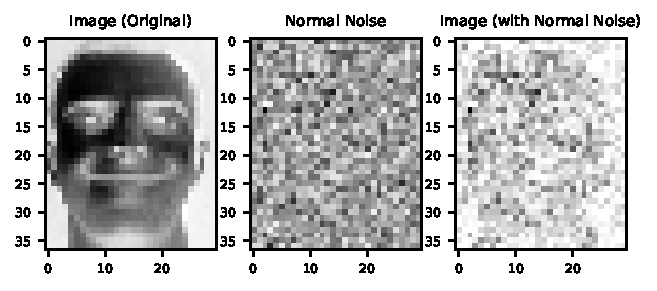
\includegraphics[scale=.8]{Noise_ORL_Normal_Comparison}\\ %replace these with jpg files with appropriate size
	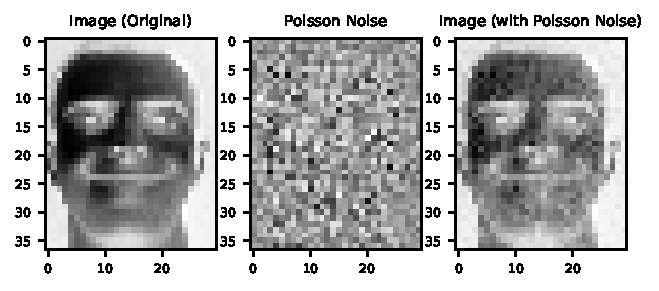
\includegraphics[scale=.8]{Noise_ORL_Poisson_Comparison}\\
	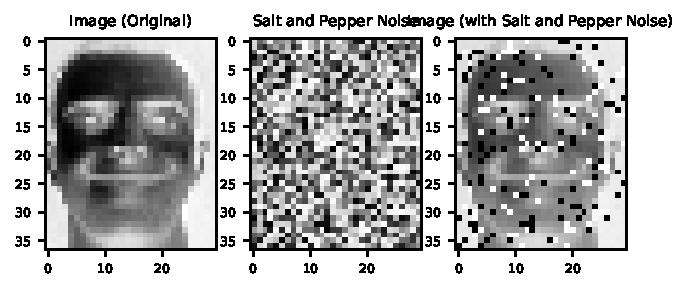
\includegraphics[scale=.8]{Noise_ORL_Salt_and_Pepper_Comparison}
	\caption{The original images (left) are corrupted by Gaussian Noise (top), Poisson Noise (middle), and Salt \& Pepper Noise (bottom). The corrupted images are shown on the right.}
	\label{fig:noise}
\end{figure}
